\documentclass[conference]{IEEEtran}
\IEEEoverridecommandlockouts
% The preceding line is only needed to identify funding in the first footnote. If that is unneeded, please comment it out.
\usepackage{cite}
\usepackage{amsmath,amssymb,amsfonts}
\usepackage{algorithmic}
\usepackage{graphicx}
\usepackage{textcomp}
\usepackage{xcolor}
\usepackage{algorithm}
\usepackage{algorithmic}
\usepackage{tabularx}
\usepackage{pgfplots}
\usepackage{multirow}
\usepackage{hyperref}

\pgfplotsset{width=10cm,compat=1.9}
\usepgfplotslibrary{external}
\tikzexternalize

\def\BibTeX{{\rm B\kern-.05em{\sc i\kern-.025em b}\kern-.08em
    T\kern-.1667em\lower.7ex\hbox{E}\kern-.125emX}}
\begin{document}

\title{Mapping transformers to compute-in-memory architectures}
\author{
 Giorgio Daneri \\
  Politecnico di Milano\\
  \texttt{giorgio.daneri@mail.polimi.it} \\

   \And
 Jacopo Palumbo \\
  Politecnico di Milano\\
  \texttt{jacopo.palumbo@mail.polimi.it} \\
}
\author{\IEEEauthorblockN{Giorgio Daneri}
\IEEEauthorblockA{\textit{Politecnico di Milano} \\
giorgio.daneri@mail.polimi.it}
\and
\IEEEauthorblockN{Jacopo Palumbo}
\IEEEauthorblockA{\textit{Politecnico di Milano} \\
jacopo.palumbo@mail.polimi.it}
}

\maketitle

\begin{abstract}
 In this article we try different mappings of transformer architectures to compute-in-memory (CIM) systems, highlighting the potential for significant improvements in efficiency and performance. Transformers have revolutionized natural language processing and various other fields with their self-attention mechanisms and parallel processing capabilities. However, their substantial computational and memory demands pose significant challenges for traditional digital computing architectures. CIM architectures offer a promising alternative by integrating memory and computation within the same hardware units, thus minimizing data transfer bottlenecks and enhancing computational throughput. 
\end{abstract}

\begin{IEEEkeywords}
Transformers, Compute-in-Memory
\end{IEEEkeywords}

\section{Introduction}
\subsection{The Compute-in-Memory (CiM) architecture}
First and foremost, let us briefly discuss the concept of computing in memory (CiM) and the advantages it brings. It is an innovative paradigm that integrates data processing capabilities directly within memory hardware, bypassing the traditional bottleneck of data transfer between memory and processors. It leverages shorter data paths, which results in minimizing latency, as well as boosting performance and energy efficiency.  
This is particularly beneficial when it comes deep neural networks (DNNs), since it avoids energy intensive weight movements and uses memory arrays to perform high-density and low-energy computations. These new architectures can accelerate AI inference by performing computations in analog format. Multiply-Accumulate (MAC) operations, which are predominant in deep learning, are optimized by reading the rows of an array of memory cells  \cite{wolters2024memory}, which can be implemented with different emerging technologies. Results are then collected along the columns of the memory array, thereby enabling parallel computation of matrix vector multiplications. Since DNNs and specifically transformers operations are centered around matrix multiplications, CiM architectures are particularly suitable for accelerating natural language processing (NLP) tasks.
Nonetheless, this process requires a major effort in designing new architectures which are specifically conceived to accelerate DNN workloads, even though this falls out outside the scope of this analysis.


\begin{figure}[ht]
    \centering
    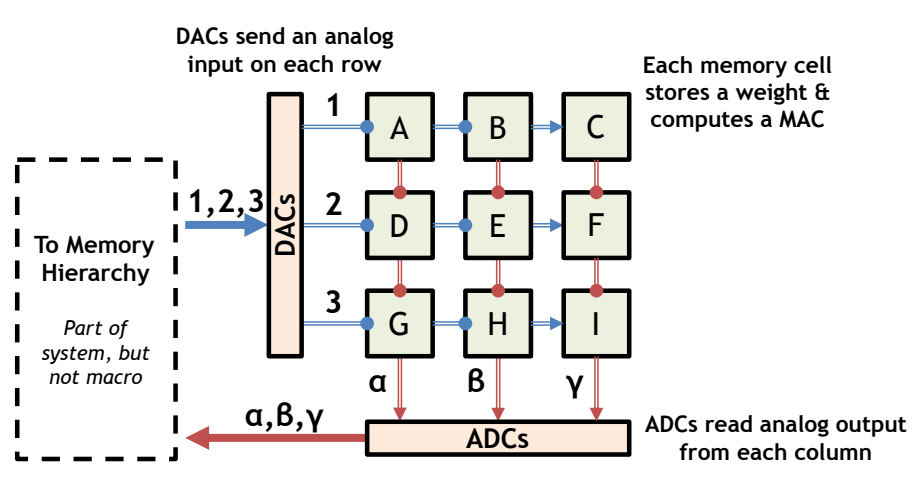
\includegraphics[width=0.3\textwidth]{images/computing_in_memory.png}
    \caption{CiM unit structure}
\end{figure}

The backbone of a CiM architecture is the set of CiM units, which are designed to perform data processing directly within the memory, integrating both computational and storage functionalities. A CiM unit features a digital to analog converter (DAC) that translates the digital signal to an analog one. Another critical component consists of the row drivers, the circuits that distribute each input element to all the corresponding elements of the array columns. This is carried out by applying the voltages produced by the DAC to the rows of the memory array \cite{andrulis2024cimloopflexibleaccuratefast}. Then the column drivers read out the analog output values from the memory array and finally the analog to digital converter (ADC) converts analog outputs from each column into digital values. This is the general structure of a CiM unit, the core component of this new architecture category.

\subsection{Overview of the transformer architecture}
Before the introduction of the transformer architecture \cite{NIPS2017_3f5ee243}, RNNs and LSTMs were mainly employed in language modeling and machine translation tasks. 
Unlike traditional RNNs and LSTMs, which process sequences of tokens sequentially, the transformer processes entire sequences simultaneously, allowing for greater parallelization and efficiency. The core innovation of the transformer lies in its use of self-attention mechanisms, which enable the model to weigh the importance of different words in a sequence relative to each other, regardless of their positions. This is facilitated by multi-head attention, which allows the model to attend to information from multiple representation subspaces at different positions. The architecture (Fig. \ref{fig:transformer_architecture}) is divided into an encoder and a decoder, both comprising stacked layers of self-attention and feed-forward neural networks, making it highly versatile and powerful for a wide range of NLP tasks, from machine translation to text generation. The introduction of positional encodings to represent the order of tokens further enhances its ability to capture sequential information. The transformer has since become the foundation for many state-of-the-art models.
\begin{figure}[ht]
    \centering
    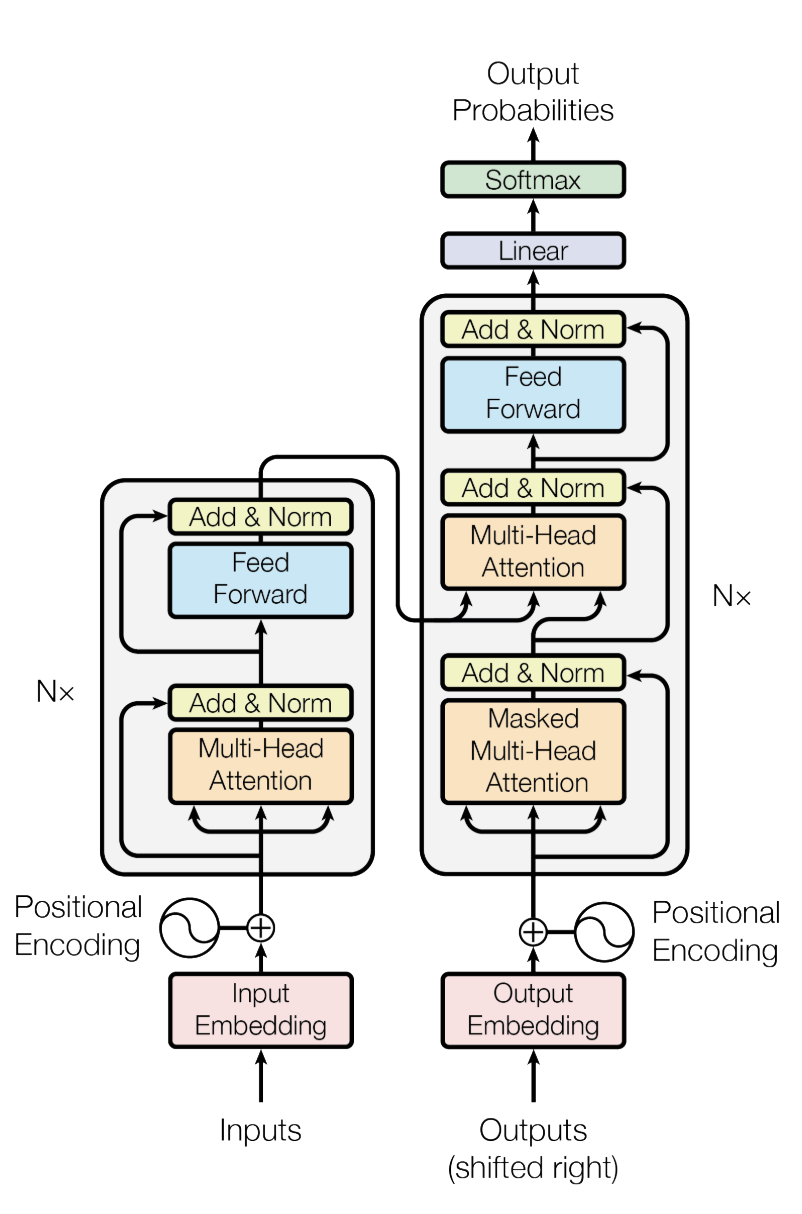
\includegraphics[width=0.3\textwidth]{images/transformer_architecture.png}
    \caption{The transformer architecture}
    \label{fig:transformer_architecture}
\end{figure}
\subsection{LLMs: decoder-only or encoder-only}
Large Language Models (LLMs) can be broadly categorized into decoder-only and encoder-only architectures, each serving distinct purposes and offering unique advantages. Decoder-only models, such as GPT (Generative Pre-trained Transformer) \cite{radford2018improving}, focus on generating coherent and contextually relevant text by predicting the next word in a sequence. These models excel in tasks like text generation and summarization. On the other hand, encoder-only models, exemplified by BERT (Bidirectional Encoder Representations from Transformers) \cite{2018arXiv181004805D}, are designed to understand and represent the input text comprehensively. They are particularly powerful for tasks requiring deep contextual understanding, such as text classification, sentiment analysis, and named entity recognition. Encoder-only models work by transforming the input sequence into a high-dimensional representation that captures intricate details and relationships within the text, enabling robust performance on various understanding tasks.

Both architectures leverage the self-attention mechanism of transformers but apply it differently to meet their respective goals. 

\section{The CimLoop Infrastructure}
CiMLoop \cite{andrulis2024cimloopflexibleaccuratefast} is a comprehensive modeling infrastructure designed to support Compute-in-Memory (CiM) systems. Built on the Timeloop+Accelergy framework, CiMLoop allows users to describe systems using YAML files for architecture, workload, and components, facilitating a seamless Python interface for running the infrastructure. Accelergy \cite{8942149} handles area and energy estimations for each component, while Timeloop \cite{8695666} leverages these estimates to perform mapping searches and model the system's energy, throughput, and area when running DNN workloads. CiMLoop enhances this foundation by introducing features specifically for CiM, including a component modeling interface for data-value-dependent modeling and support for circuit-level data movement and reuse. It also introduces a flexible architecture specification and a fast modeling pipeline, enabling accurate and efficient evaluation of design decisions across all levels of the CiM stack.

\section{Proposed CiM architectures}
CiMloop offers several architectures that model the hardware components with different precision levels. While they weren't designed specifically for transformers, they can still achieve good performance and efficiency since the basic operations are matrix multiplications, which are ubiquitous in the DNNs world. The standard architecture is called Basic Analog, though it is not of our interest due to its oversimplification of the hardware details; it does not model important components, so the overall energy consumption is far from what would be observed in reality. We rather focus on three high-fidelity architectures that have been published in academic journals:
\begin{itemize}
    \item NeuRRAM architecture \cite{wan2022compute}, a CiM chip based on resistive random access memory (RRAM), featuring 48 cores, that simultaneously delivers versatility in reconfiguring CiM cores for diverse model architectures, energy efficiency that is two-times better than previous state-of-the-art RRAM-CiM chips across various computational bit-precisions, as well as inference accuracy comparable to software models quantized to four-bit weights across various AI tasks. At the device level, 3 million RRAM devices
    with high analogue programmability are integrated
    with CMOS circuits. At the circuit level, a voltage-mode neuron
    circuit supports variable computation bit-precision and activation functions while performing analogue-to-digital conversion at low
    power consumption and compact-area footprint. At the system
    level, 48 CIM cores can perform inference in parallel and supports
    various weight-mapping strategies. Note that a core can be selectively turned off through power gating when not actively used, whereas the model weights are retained by the non-volatile RRAM devices.

    \item Sinangil architecture \cite{sinangil20207}, which utilizes a 7-nm FinFET technology and is based on SRAM technology. The main features of this architecture include support for 4-bit inputs, weights, and outputs, enabling efficient multiply-and-accumulate (MAC) operations. Specifically, it can perform 1024 4-bit × 4-bit MAC operations simultaneously. The design employs a standard two-port compiler macro using an 8T bit-cell, incorporating ADCs and charge-sharing mechanisms for computation, which saves area and reduces kick-back effects. The 7-nm technology allows for high density and performance. Macro size is chosen as proof-of-concept and amenable to realize larger weight matrices by combining multiple macros, which tends to perform better than a single large macro. This work supports 4-b inputs, 4-b weights, and 4-b outputs. 4-b inputs are realized using a series of unit read word-line (RWL) pulses. This is implemented by placing  counters and necessary RWL drivers, weights are realized by sampling RBL voltage on binary-weighted capacitors and doing charge sharing to combine column-wise 1-b MAC results in a weighted fashion. Lastly, 4-b output is generated through a 4-b Flash ADC.

    \item Colonnade architecture \cite{kim2021colonnade}, a fully digital, static RAM (SRAM) based, bit-serial CiM macro. It features a regular digital bitcell array that is readily reconfigured to a 1–16 bit weight-stationary bit-serial CIM macro. A column of bitcells forms a column MAC and is used for computing a multiply-and-accumulate (MAC) operation. The column MAC is placed in a row work as a single neuron and computes a dot-product, which is an essential building block of neural network accelerators. Its full-digital circuit implementation is free from process variation, noise susceptibility, and data-conversion overhead that are prevalent in prior analog CIM macros. A bitwise MAC operation in a bitcell is performed in the digital domain using a custom-designed XNOR gate and a fulladder. The macro computes parallel dot-product operations between the weights stored in memory and inputs that are serialized from LSB to MSB. Finally, the bit-serial computing scheme significantly reduces the overhead while sacrificing latency due to bit-by-bit operation cycles. Based on the benefits of digital CIM, reconfigurability, and bit-serial computing architecture, the Colonnade can achieve both high performance and energy efficiency.
\end{itemize}

The main difference between the first two architectures and the last one is that the former perform computations in analog format, while the latter is fully digital. For this reason, Colonnade does not contain any ADC or DAC components. Performing computations in digital format offers higher precision (Colonnade supports up to 16 bit precision, higher than that of the other two architectures) and more resilience with respect to noise. Error detection and correction mechanisms are also more readily available and easily applicable to digital signals rather than to analog ones. While static power consumption is low for digital circuits, analog circuits can offer extremely lower dynamic power consumption, which is pivotal when trying to achieve high energy efficiency. The implementation choice has huge impacts on the power consumption of the macro, as we will conclude from the workload mapping process.
%Another important difference is the die area of the chips. The NeuRRAM chip is more %complex and powerful, thus it occupies more space and is capable of handling bigger %workloads. The dimensions of the chip are $10.8\times14.7mm$, which amounts to $158.76 %mm^2$, while a single core has an area of $1mm^2$. The latter chip... 
\section{Proposed LLMs}
In this analysis we focus on the decoder-only architecture (GPT-like LLMs) with the objective of finding the best tuple CiM-LLM to employ LLMs inference on the edge.

The experimental set is composed by the following LLMs:
\begin{itemize}

\item GPT-2 Medium \cite{radford2019language}: designed by OpenAI, features a model with 345 million parameters, structured to balance performance and computational efficiency. This version of GPT-2 includes 24 transformer decoder layers, each designed to capture complex patterns in the input data.

Each layer in the medium GPT-2 model consists of a multi-head self-attention mechanism, which enables the model to focus on different parts of the input sequence simultaneously, allowing it to capture various dependencies and relationships between words. The medium model uses 16 attention heads in each layer, facilitating the parallel processing of information.

Following the attention mechanism, each layer includes a position-wise feed-forward neural network (FFN), which consists of two linear transformations with a ReLU activation in between. This helps to model complex patterns and interactions in the data. The hidden dimension of the FFN in the medium model is 1024.

Layer normalization is applied both before the multi-head attention mechanism and the feed-forward network, which helps stabilize and accelerate training by normalizing the inputs to each sub-layer, maintaining mean and variance. Each sub-layer (attention and FFN) also has a residual connection around it, aiding in training deep networks by allowing gradients to flow more easily through the network.

\item Phi-3 \cite{abdin2024phi}: designed to balance performance and efficiency, especially in small to medium-scale models. The core model, Phi-3-mini, is a transformer decoder architecture with a default context length of 4K, extendable to 128K via LongRope \cite{ding2024longrope} for specific variants. It employs a hidden dimension of 3072, 32 heads, and 32 layers. The model uses a 320641 token vocabulary, benefiting from its compatibility with the Llama-2 family, allowing seamless adaptation of existing Llama-2 resources.

This model introduces enhancements like switching from GELU to GEGLU activation and using Maximal Update Parametrization (muP) for hyperparameter tuning, which ensures better training stability and performance. Additionally, it incorporates a novel blocksparse attention mechanism, optimizing training and inference efficiency by enforcing different sparsity patterns over the KV cache and alternating dense and blocksparse attention layers.

Overall, the Phi-3 architecture focuses on maximizing efficiency and performance through innovative training methodologies, effective parameter tuning, and advanced attention mechanisms, making it suitable for a range of applications from mobile deployment to more extensive, resource-intensive tasks.

\item Mistral 7B \cite{jiang2023mistral}: a 7-billion-parameter language model designed for high efficiency and performance. It uses a transformer architecture with several innovations, including Grouped-Query Attention (GQA) to improve inference speed and reduce memory requirements, and Sliding Window Attention (SWA) to handle long sequences effectively. The model features an embedding dimension of 4096, 32 layers, a hidden dimension of 14336, 32 attention heads, and 8 key/value heads, with a context length of 8192 tokens and a vocabulary size of 32,000. These design choices enable Mistral 7B to outperform larger models like Llama 2 13B, particularly in tasks involving reasoning, mathematics, and code generation, while maintaining efficient memory usage and fast inference speeds.

Mistral 7B's architectural enhancements, such as the rolling buffer cache and pre-fill with chunking, further optimize its handling of long sequences by managing memory efficiently and reducing the quadratic complexity of traditional attention mechanisms. This balance of computational efficiency and performance makes Mistral 7B suitable for real-time applications and deployment in resource-constrained environments, offering a powerful yet resource-efficient solution for a wide range of natural language processing tasks.

\item Llama 2 \cite{touvron2023llamatwo}: built upon the original LLaMA \cite{touvron2023llama} with several enhancements aimed at improving performance and efficiency. Key architectural changes include an expansion of the context window from 2048 to 4096 tokens, enabling the model to handle longer sequences, which is particularly beneficial for tasks requiring extensive context such as long document summarization and chat applications.

The model employs a Grouped-Query Attention (GQA) mechanism, which helps to manage the increased memory costs associated with larger context windows and batch sizes. This approach involves sharing key and value projections across multiple heads, thus reducing the KV cache size without significantly degrading performance.

LLaMA 2 retains the transformer architecture, with specific configurations across different model sizes (7B, 13B, and 70B parameters). The architecture typically includes multiple transformer blocks, each comprising multi-head self-attention layers and feed-forward neural networks. The feed-forward layers and the attention heads have dimensions that are scaled according to the model size, ensuring a balance between capacity and computational efficiency. In our experiments we used the 7B model. 
\end{itemize}

\subsection{Why only inference?}
Mapping only transformer inference to compute-in-memory (CIM) architectures is primarily driven by the substantial hardware and energy demands associated with the training phase. Training transformers involves processing massive datasets through numerous iterations, requiring extensive computational power and memory bandwidth. This process is both time-consuming and resource-intensive, necessitating large-scale, specialized hardware like GPUs or TPUs to manage the colossal amount of matrix multiplications and gradient calculations efficiently. In contrast, inference, which is the application of a trained model to new data, is comparatively less demanding. CIM architectures, which integrate computation and memory storage to reduce data transfer bottlenecks and enhance efficiency, are particularly well-suited for the fixed and predictable nature of inference tasks. By focusing on inference, CIM systems can leverage their strengths in energy efficiency and speed without the overwhelming resource requirements of training. Additionally, the deployment of transformer inference on CIM architectures aligns well with the principles of edge computing, where computational tasks are performed closer to the data source to minimize latency and bandwidth usage. This strategic allocation allows for more practical and cost-effective deployment of transformer models in real-world applications, enabling the benefits of advanced AI with significantly reduced hardware and operational costs while enhancing performance in edge devices.

\subsection{Practical approach}
We used the PyTorch library to load the models and access the layers, as well as to produce the histograms relative to the distribution of the input, output and weight values. We leveraged the remote resources offered by Google Colab and moved the storage and calculations to the GPU, which offers acceleration with the CUDA library. Producing the histograms is fundamental in order to model the power consumption of the various layers, especially when the workload is mapped on an analog architecture. The more the values of the matrices are clustered around the zero, the lower the expected energy consumption. This is because a value is codified as a tension when it is converted to analog format by the DAC; the higher its absolute value, the higher the tension necessary to represent it in the memory cell. This reasoning does not directly apply to the Colonnade architecture, which is fully digital. It is therefore more complex to understand the factors that contribute to energy consumption in the case of this architecture. 

\begin{figure}[ht]
    \centering
    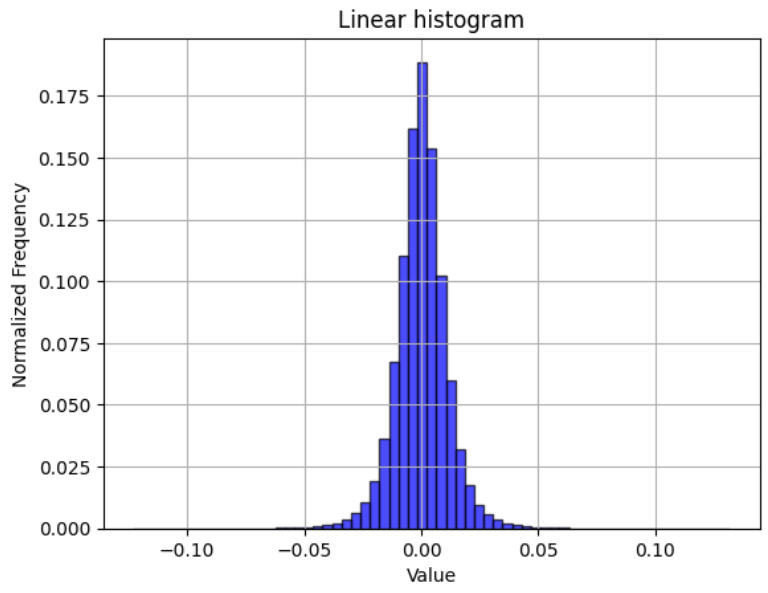
\includegraphics[width=0.4\textwidth]{images/histogram_llama2.png}
    \caption{Weight distribution of Llama2 linear layer}
    \label{fig:llama2_hist}
\end{figure}

All the histograms are centered around the origin and are normalized to unity, thus they constitute a probability distribution of the values. We used 64 bins to achieve high precision in the value distribution. 
In order to extract the workload, we considered only the linear (feed-forward) and attention layers, which correspond to the vast majority of computations, thus of the energy consumption. The other layers, especially the non-linear ones, require a non-trivial mapping to the CiM architecture that goes beyond the scope of this analysis. This is because CiM architectures are conceived for MAC operations, which are intrinsically linear. Moreover, their impact is limited and we can therefore exclude them from the workload without introducing too big an approximation. As for the attention layers, we needed to extract namely the projections of the input embeddings into the key, query and value matrices.
Then the necessary information is formatted in a sequence of YAML files, one per each layer. A single file describes the dimensions of the input and output features and contains the histograms of the input, output and weight matrices in the form of arrays. 

All the Python scripts to generate the histograms and produce the workloads in the YAML format are available in the github repository at \hyperlink{this link}{https://github.com/giorgiodaneri/ACA\_project}

\section{The experimental results}
We used a Cimloop function to perform a full DNN exploration of some workloads corresponding to both older and state-of-the-art transformers. These include the aforementioned GPT2, Phi-3, Llama-2 and Mistral. We mapped them on the three architectures described above, among those already available on Cimloop. 
On the x-axis we reported the number of layers of the workload, while on the y-axis we depicted the energy consumption in femto Joules per MAC operation (1e-15 J/MAC). The input sequence is 10 tokens, thus very short. In order to produce the histograms, we limited the output length to a single token so that each layer is visited exactly once.
First let us analyze one of the main ancestors of the current state-of-the-art transformers, GPT2 medium, consisting of 144 layers (1D convolutional and attention layers). 

In all three plots (\ref{fig:gpt2_wan}) (\ref{fig:gpt2_sinangil}) (\ref{fig:gpt2_colonnade}) we can notice periodic peaks, corresponding to the attention layers, whose power consumption is remarkably higher than that of the convolutional layers. The result is realistic since these layers handle heavy algebraic computations due to high-dimensionality weight matrices. Though actual power consumption depends on many factors, such as the sparsity pattern of the matrices involved as well as the input sequence length. To understand this is greater depth, we need to consider the theoretical computational complexity of the two operations. The self-attention mechanism has a computational and memory complexity of $O(d \cdot n^2)$ \cite{fournier2023practical}, where $d$ is the dimension of the token embeddings and $n$ is the input sequence length. On the other hand, the computational complexity of the conv1D operation is $O(k \cdot n \cdot d^2)$ \cite{NIPS2017_3f5ee243}, where $k$ is the length of the filter. Clearly, in this case the input sequence $n$ dominates the overall complexity, resulting in attention layers consuming more power. \\

Then we shall move onto analyzing Phi-3 and look for similarities and differences between the experimental results. Note that this architecture does not contain Conv1D layers, which are replaced with linear (feed-forward) layers. Since this transformer is the most recent and can be considered state-of-the-art, this analysis will be conducted in deeper detail. 
For the first two plots (\ref{fig:phi3_wan}) (\ref{fig:phi3_sinangil}), we observe again a dominance of the attention layers. In the first case, the dominant components are the CiM unit, the integrator, the row drivers and the wordline capacitors. The CiM unit is expected to consume an important portion of the total energy, since it acts both as storage and computational unit. In the context of ReRAM architectures, the integrator is used to perform matrix-vector multiplications. It accumulates the weighted sums of input signals, which are typically voltages or currents, representing the matrix and vector elements respectively. Analog integrators can help in smoothing out the noise inherent in analog computations, leading to more accurate results. By integrating the signal over time, transient noise and fluctuations can be averaged out, providing a cleaner output. Finally, the wordline capacitors help manage the analog voltages applied to the wordlines (WLs), ensuring stable and precise operations during these computations. This stability and precision are necessary for maintaining the accuracy and efficiency of the analog-to-digital conversions and the overall processing within the NeuRRAM architecture.

On the other hand, the third plot (\ref{fig:phi3_colonnade}), depicting the mapping on the Colonnade macro, depicts a different result, with linear layers being the most energy intensive. The computational complexity of this operation is $O(d^2 \cdot n)$, since it involves two dense layers with a SiLU activation function in between. Due to the input sequence being very short, it is not clear which operation dominates the overall energy consumption. The linear layer consumption also depends on the dimensions of the input and output features, which appear to be the most influential ones. Though this fully digital architecture has a significantly different behaviour with respect to standard analog CiM macros. The hardware component which dominate in this case are the column drivers, which serve a purpose similar to that of the integrator in NeuRRAM, followed by the CiM logic and CiM unit, as expected. Of course there is no component necessary to convert the signal from digital to analog and viceversa, since this macro is fully digital. To confirm its different energy profile it is sufficient to compare it with the first two plots, which both stem from executing a workload on analog CiM macros, NeuRRAM and Sinangil respectively. Nonetheless, the energy consumption of the second is two orders of magnitude lower than that of the first and three with respect to that of third, which is a huge improvement. The explanation could be a combination of advanced and miniaturized technology for implementing the hardware logic, which leverages 7nm transistors, and the use of a low precision format, which is limited to 4 bits (against the 8 bits for the input and 10 bits for the output of NeuRRAM and 16 bits of Colonnade).
The most consuming components are the row drivers, which are necessary to distribute each input element to all the corresponding elements of the array columns. It is unexpected to see that the contribute of the CiM unit is negligible. A possible explanation could be the underestimated consumption of this component when it is modelled inside the CiMLoop infrastructure.  In facts, CiMLoop provides a standard description for the CiM unit, no matter the actual architecture. The energy profile of this component should be modelled in accordance with the actual technology that is used to implement it, which is decisive in achieving high energy efficiency. For the reasons above, we cannot fully trust the estimates that we gathered, which should be intended as an general analysis on the architecture design and the technologies used.  

Now let us analyze the Mistral workload mapped on the same three architectures. Once again we can observe that, in the case of analog macros (\ref{fig:mistral_NeuRRAM}) (\ref{fig:mistral_Sinangil}), the most consuming layers are those corresponding to attention. As before, the Colonnade macro (\ref{fig:mistral_colonnade}) produces a different result, where linear layers consume the most. We are comforted by the fact that scaling up the LLM size, in this case from 161 to 289 layers, yields consistent results. This is to be expected since the backbone of a decoder-only transformer architecture is standardized, while the training phase makes most of the difference. GPT2 had different outcomes when mapped on the Colonnade architecture, but is also quite older (three or more years) and is constituted by different operations, so it should not be taken into consideration when looking for similarities with more recent transformers. 

The last transformer we are going to analyze is Llama2, which actually has the same layers of Mistral, as well as the same disposition. It is interesting to check whether the different internal implementation and training impacts the energy consumption or not. As we can observe from the plots (\ref{fig:llama2_NeuRRAM}) (\ref{fig:llama2_Sinangil}) (\ref{fig:llama2_Colonnade}), there is indeed a notable difference between the two workloads. We do not see a clear predominance of the attention layers for the NeuRRAM and Sinangil architectures, where the highest energy consumption peaks are located at layers 25 and 151 in both cases. Both these layers have a high number of input features, which may be the cause of such consumption. Though the overall average energy consumption is approximately the same for the two workloads, Llama2 and Mistral, no matter the pattern variations. Nevertheless, the smaller periodic peaks still correspond to attention layers. 
We can conjecture that, since the underlying architecture is almost identical for both Mistral and Llama2, the training phase is crucial to understand the power consumption of each layer, especially due to the distribution of the weight values. Of course there may be notable differences in implementation details in each layer, which too contribute to the dissimilarities. 

\subsection{The approximation introduced by CimLoop}
The histograms used by CimLoop during the mapping of the workloads carry only information regarding the distribution of the value of the parameters. The parameter distribution alone does not provide a complete picture of the energy consumption because the actual voltage levels that correspond to these parameter values are crucial in determining the power usage. The analog nature of CiM architectures means that each parameter value, represented by a specific voltage, directly influences the amount of power consumed during computation. Consequently, without precise knowledge of the voltage range (i.e., the maximum and minimum parameter values), any energy consumption estimation will be inherently imprecise.

Moreover, this limitation implies that different layers within the same model could have vastly different energy requirements based solely on the magnitude of their parameters. For instance, layers with predominantly small parameter values will inherently draw less power compared to layers with larger parameter values. This variation is not captured by simply looking at the parameter distribution, leading to potential inaccuracies in energy consumption predictions.

Therefore, while CimLoop provides valuable insights into which CiM architecture might be the most suitable for a given workload, it is important to interpret these results with caution. The primary utility of these results lies in comparative analysis rather than precise quantification. Practitioners should use CimLoop’s findings to identify promising architectural candidates and then conduct more detailed analyses, possibly incorporating additional information about parameter values and their corresponding voltages, to achieve accurate energy estimations.
\section{Conclusion}
We mapped various transformer architectures on different CiM macros, which are representative of divergent approaches to achieving high energy efficiency and compactness to enable LLM inference on the edge. We should keep in mind that these were not designed specifically for transformers, but rather for convolutional neural networks. The results obtained draw a counterintuitive conclusion, since SRAM seems to perform better than RRAM, provided that energy consumption estimates made in CiMLoop are trustworthy. In general, the opposite is true, since RRAM is more power efficient, particularly in terms of standby power consumption. Moreover, RRAM generally consumes less energy for write operations compared to SRAM, though this can vary based on the specific RRAM technology and implementation. On the other hand, SRAM grants the fastest data access and processing speeds, despite its higher energy consumption. Ultimately, it is not clear why the Sinangil macro, based on SRAM, performs better than NeuRRAM in terms of power consumption. On the other hand, we can establish a clear result about whether to choose a fully digital or analog architecture. While the former may offer several advantages in terms of precision, the rise of quantization techniques applied to DNNs makes it a secondary goal. From a power consumption perspective, working in analog format achieves unmatched results and paves the way to future research in this direction. 
When it comes to the energy consumption of different layers, we notice a general dominance of attention layers, which enclose heavy matrix multiplications with high dimensionality. In years to come, it is fundamental to design new CiM macros that are tailor made for accelerating transformer architectures in a power efficient way, focusing on mapping the multi-head attention modules on dedicated hardware, in order to optimize the most computationally intensive portion of transformers.

% TODO: compare the different macros also in terms of area consumption, since compactness is crucial on the edge. Also complete the part relative to this in the proposed architectures section

\onecolumn
\begin{center}
\begin{figure}[ht]
    \centering
    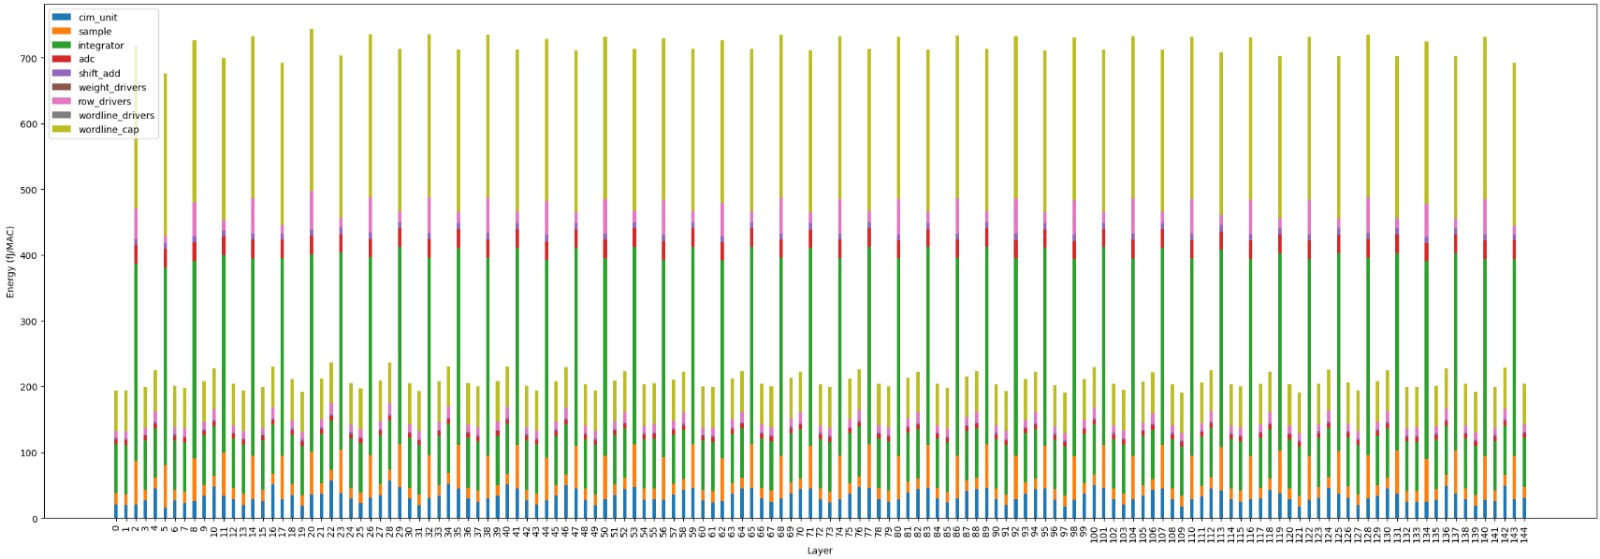
\includegraphics[width=0.85\textwidth]{images/gpt2_wan_arch.jpg}
    \caption{GPT2 on NeuRRAM architecture}
    \label{fig:gpt2_wan}
\end{figure}

\begin{figure}[ht]
    \centering
    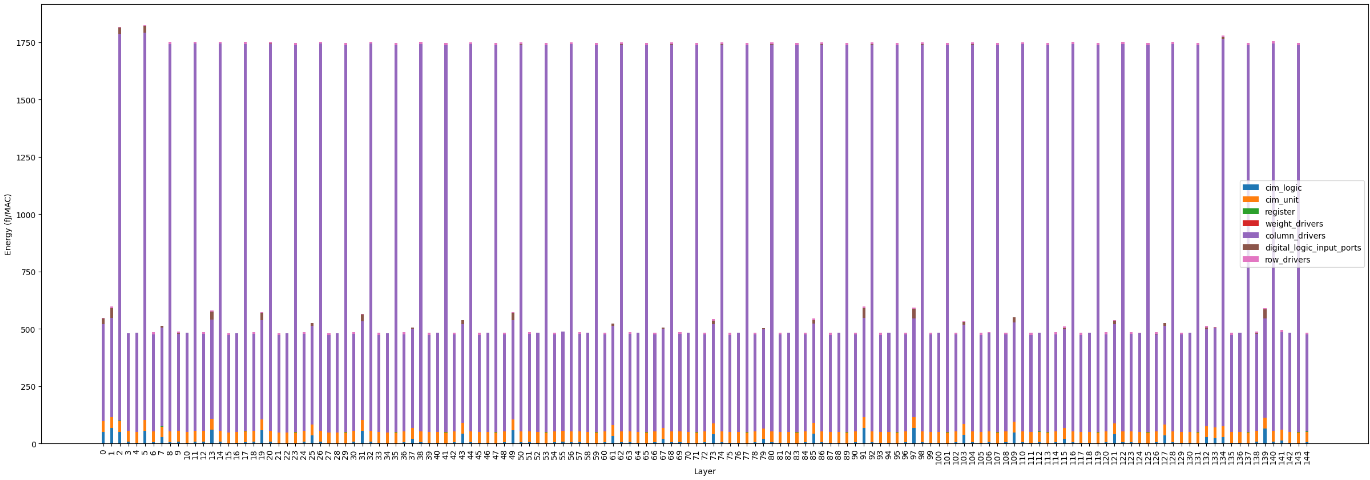
\includegraphics[width=0.85\textwidth]{images/gpt2_colonnade.png}
    \caption{GPT2 on Colonnade architecture}
    \label{fig:gpt2_sinangil}
\end{figure}

\begin{figure}[ht]
    \centering
    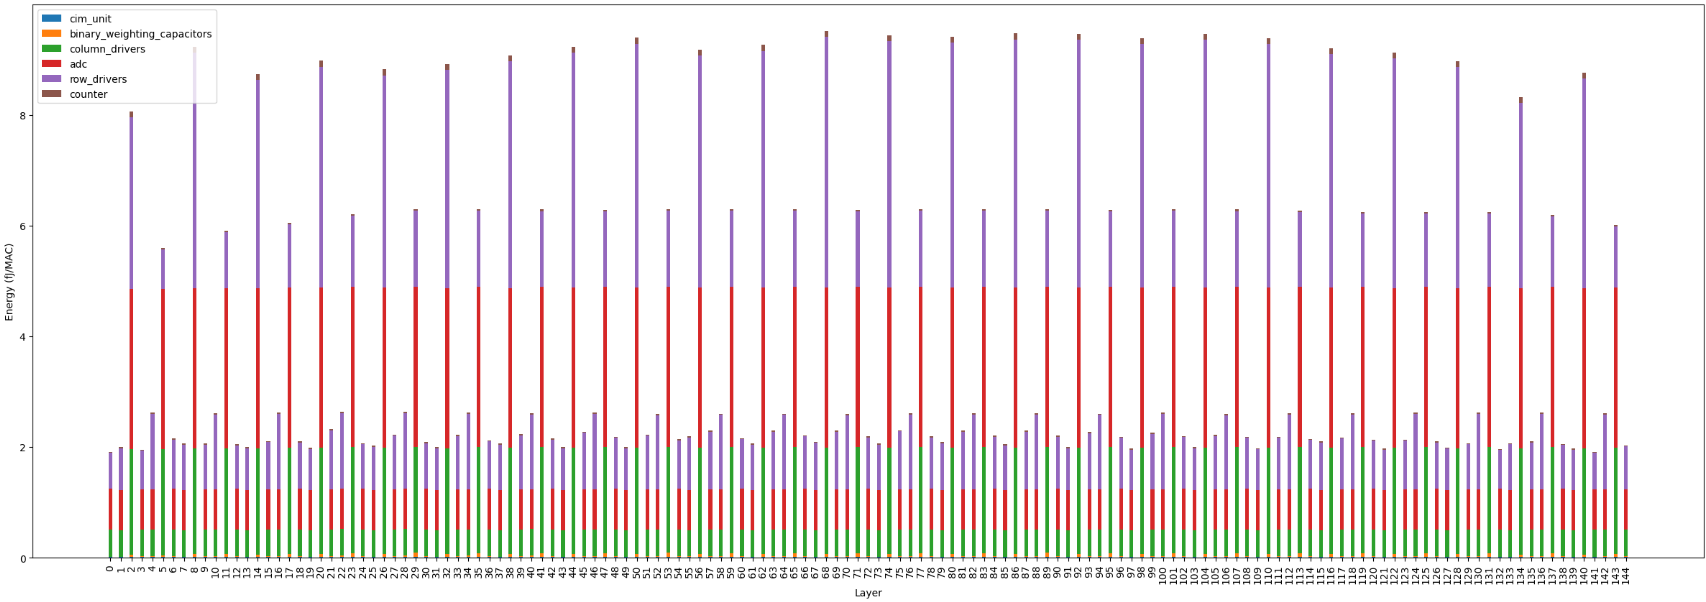
\includegraphics[width=0.85\textwidth]{images/gpt2_sinangil.png}
    \caption{GPT2 on Sinangil architecture}
    \label{fig:gpt2_colonnade}
\end{figure}

\begin{figure}[ht]
    \centering
    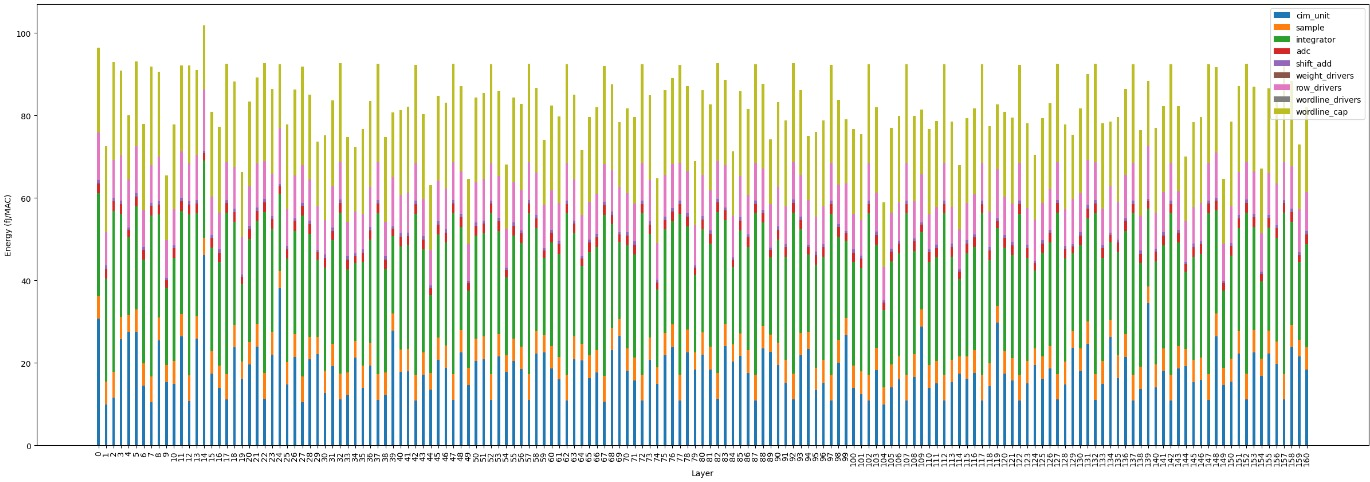
\includegraphics[width=0.9\textwidth]{images/phi3_wan_arch.jpg}
    \caption{Phi-3 on NeuRRAM architecture}
    \label{fig:phi3_wan}
\end{figure}

\begin{figure}[ht]
    \centering
    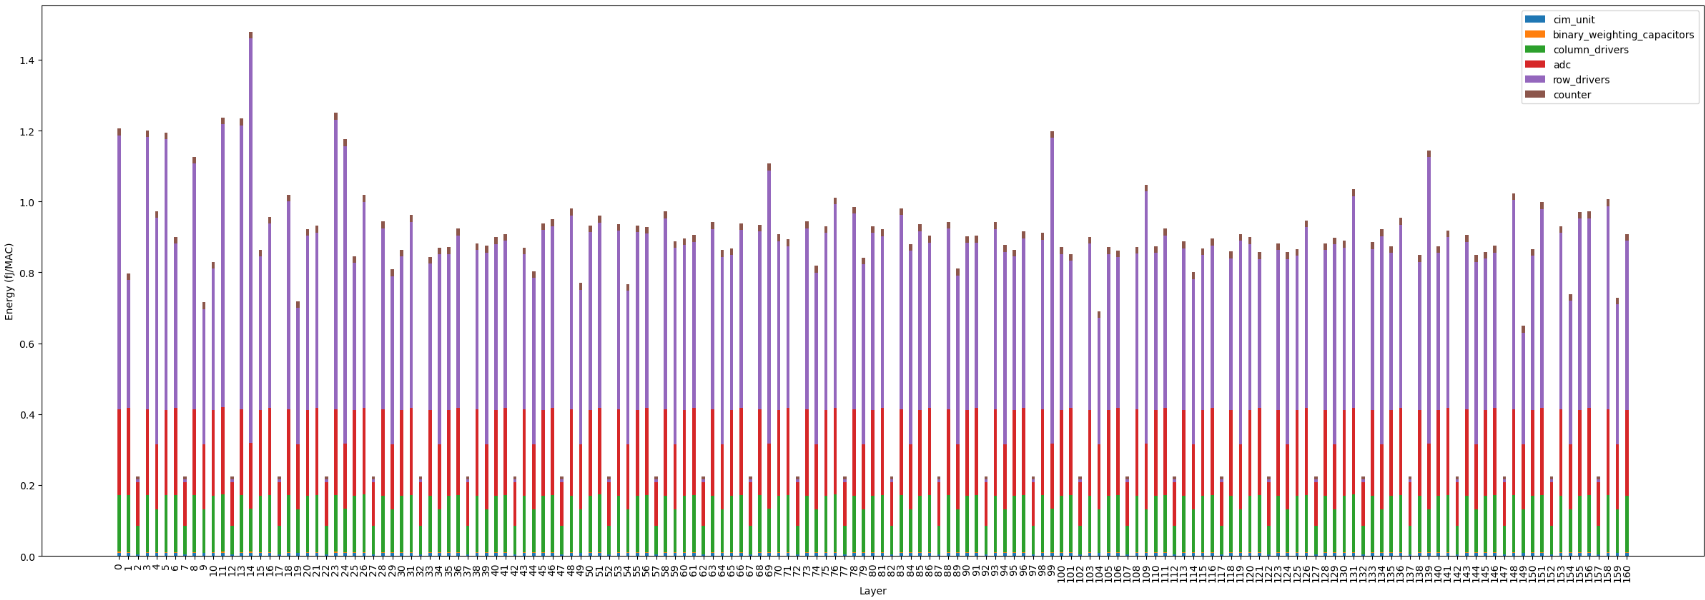
\includegraphics[width=0.9\textwidth]{images/phi3_sinangil.png}
    \caption{Phi-3 on Sinangil architecture}
    \label{fig:phi3_sinangil}
\end{figure}

\begin{figure}[ht]
    \centering
    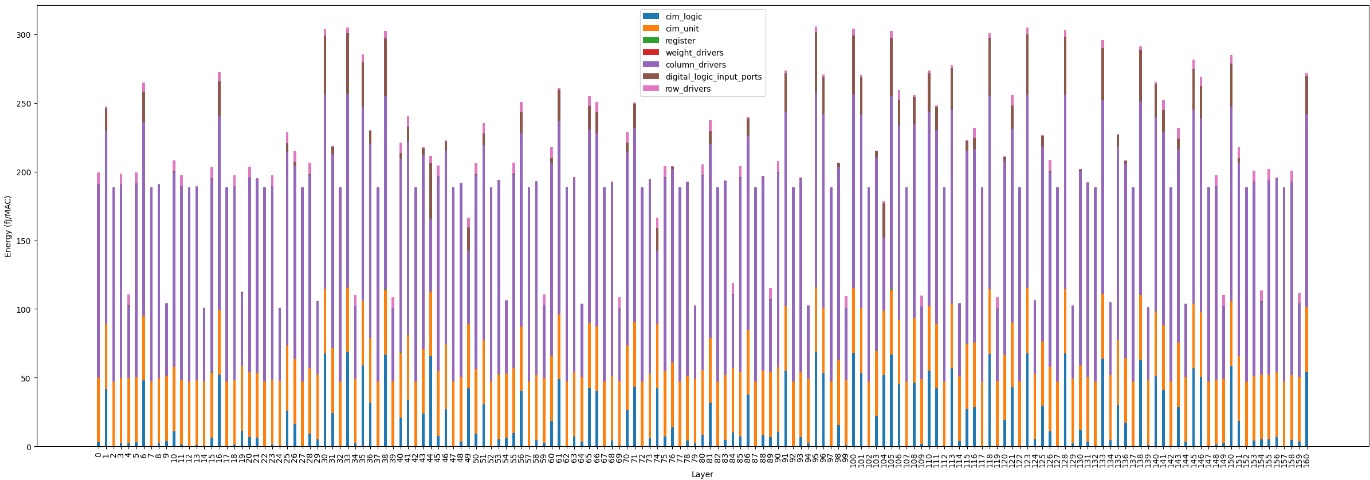
\includegraphics[width=0.9\textwidth]{images/phi3_colonnade_arch.jpg}
    \caption{Phi-3 on Colonnade architecture}
    \label{fig:phi3_colonnade}
\end{figure}

\begin{figure}[ht]
    \centering
    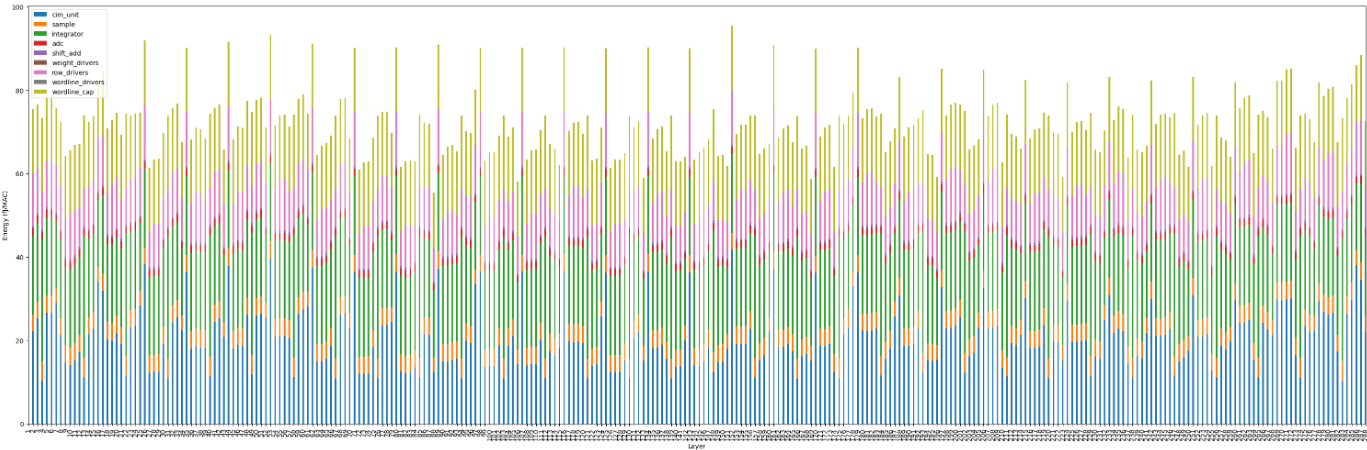
\includegraphics[width=0.9\textwidth]{images/mistral_wan_arch.png}
    \caption{Mistral on NeuRRAM architecture}
    \label{fig:mistral_NeuRRAM}
\end{figure}

\begin{figure}[ht]
    \centering
    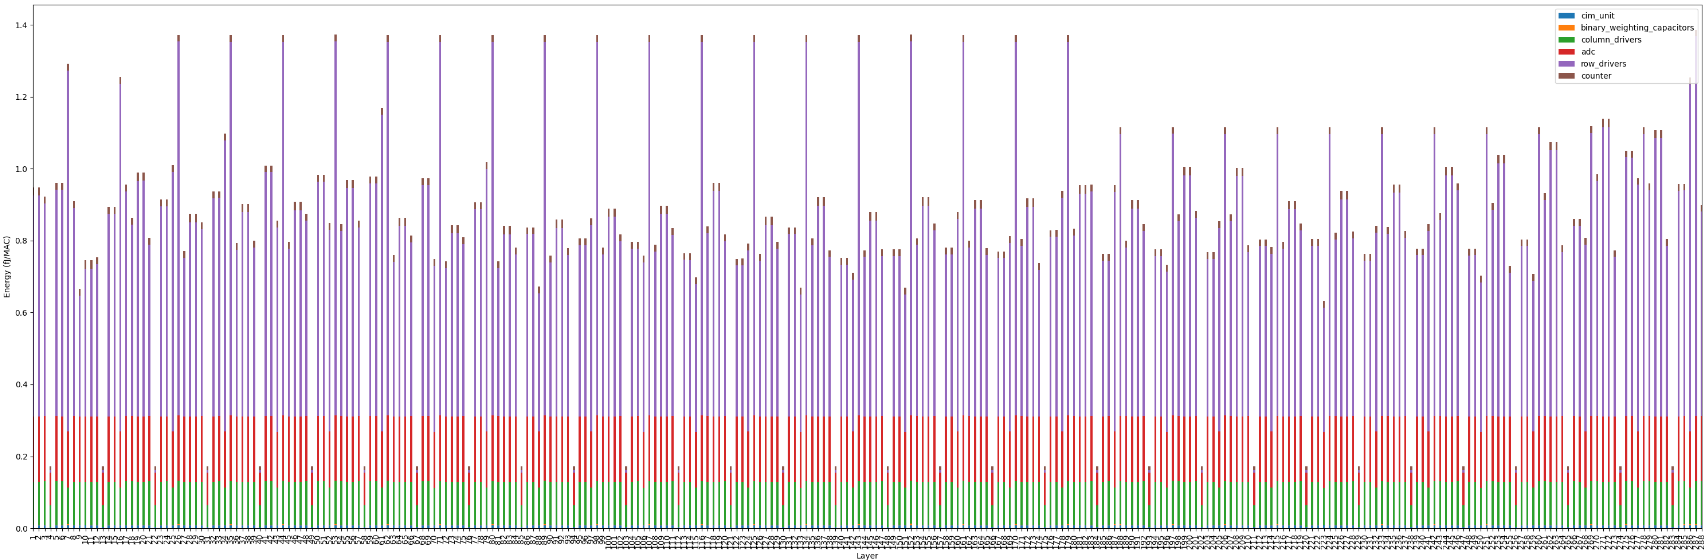
\includegraphics[width=0.9\textwidth]{images/mistral_sinangil_arch.png}
    \caption{Mistral on Sinangil architecture}
    \label{fig:mistral_Sinangil}
\end{figure}

\begin{figure}[ht]
    \centering
    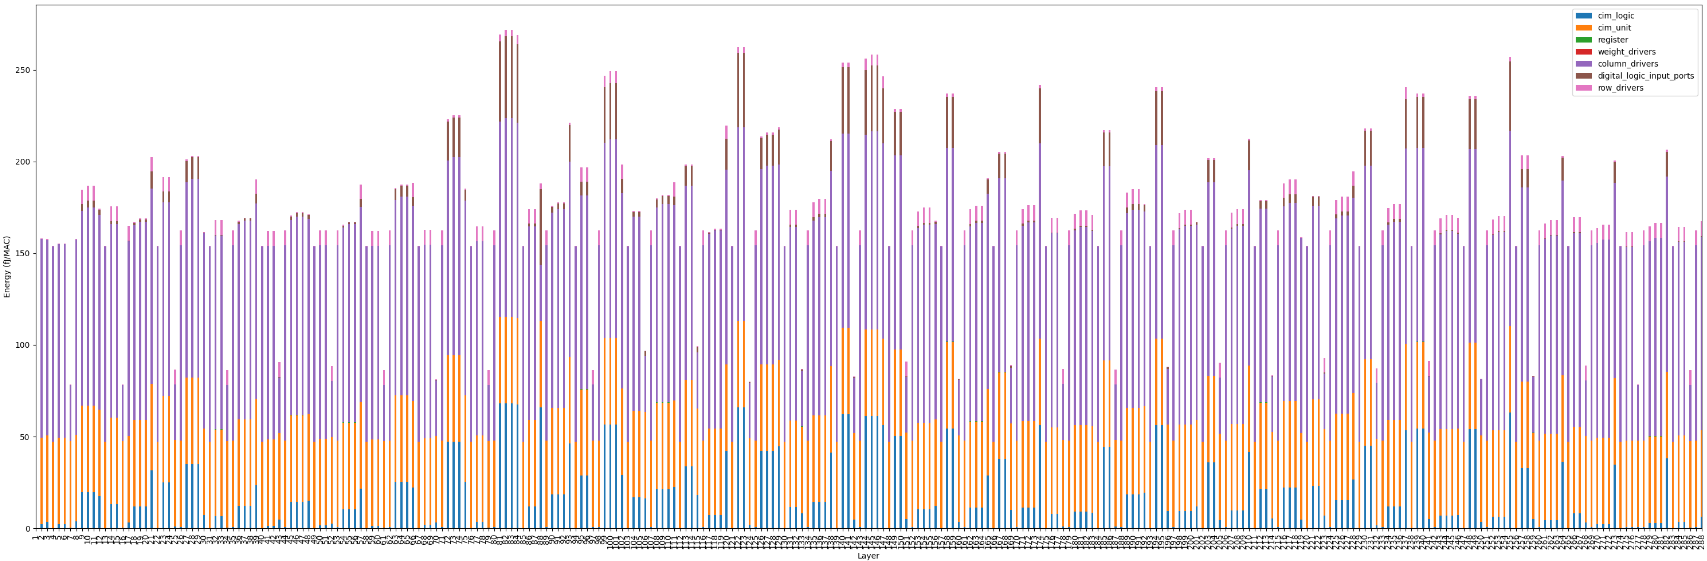
\includegraphics[width=0.9\textwidth]{images/mistral_colonnade_arch.png}
    \caption{Mistral on Colonnade architecture}
    \label{fig:mistral_colonnade}
\end{figure}

\begin{figure}[ht]
    \centering
    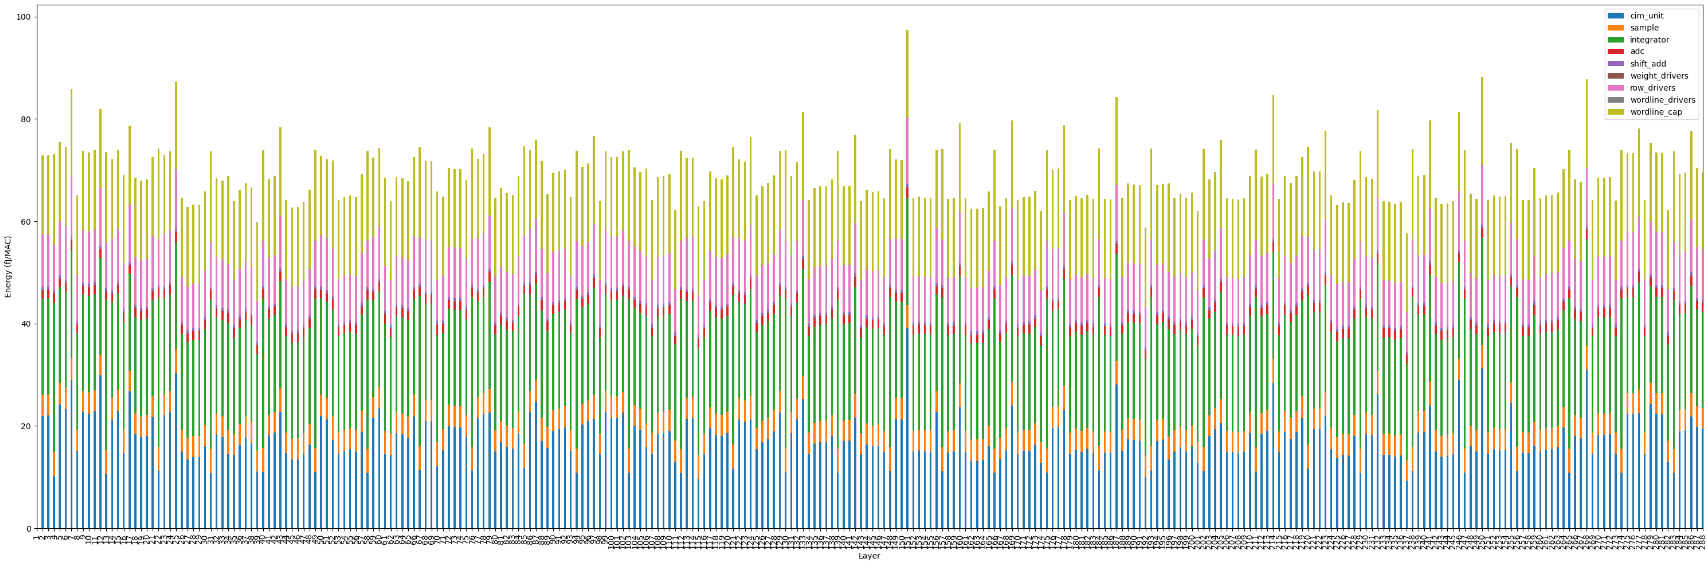
\includegraphics[width=0.9\textwidth]{images/llama2_wan_arch.png}
    \caption{Llama2 on NeuRRAM architecture}
    \label{fig:llama2_NeuRRAM}
\end{figure}

\begin{figure}[ht]
    \centering
    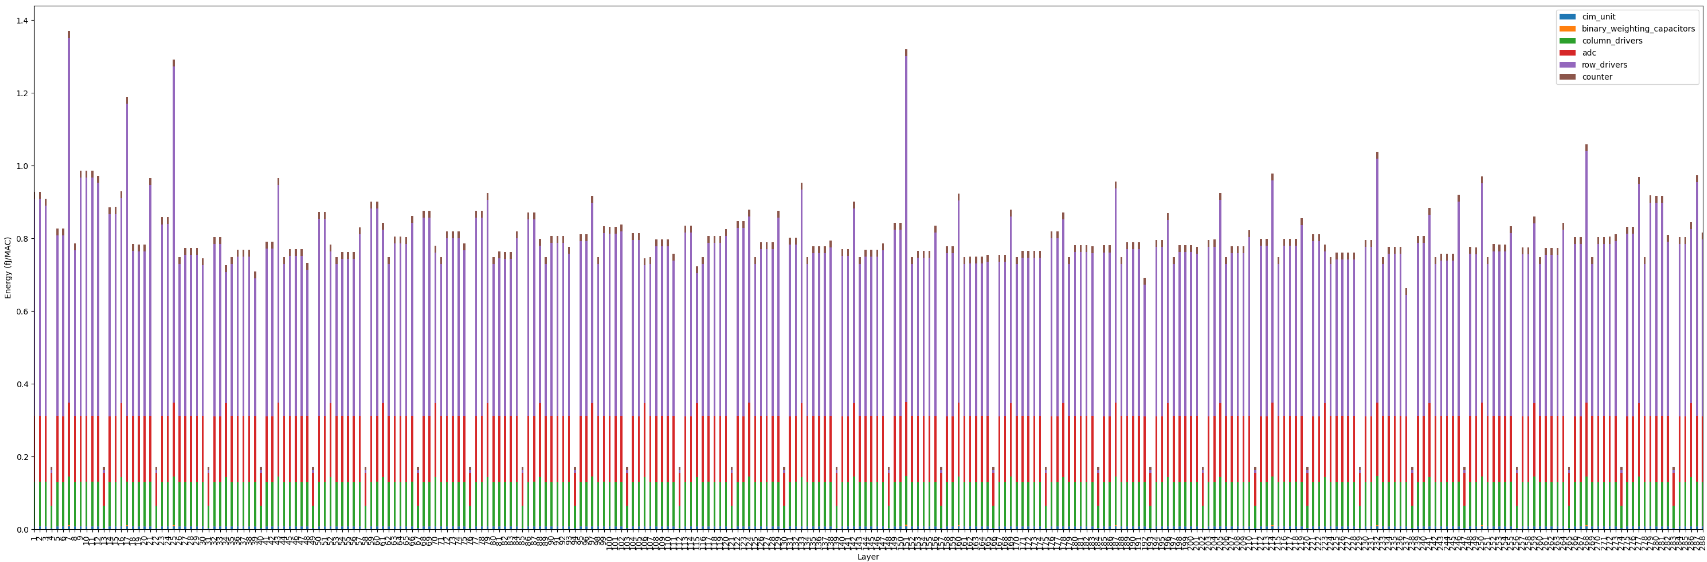
\includegraphics[width=0.9\textwidth]{images/llama2_sinangil.png}
    \caption{Llama2 on Sinangil architecture}
    \label{fig:llama2_Sinangil}
\end{figure}

\begin{figure}[ht]
    \centering
    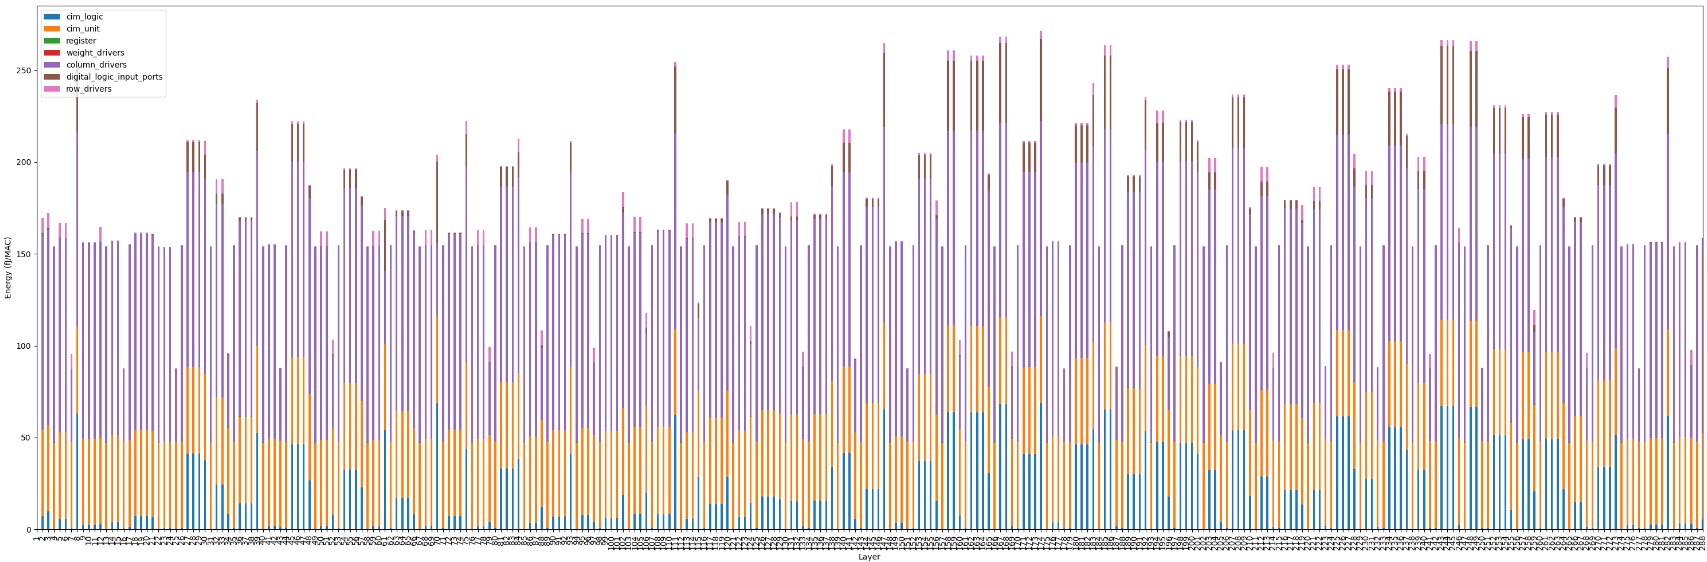
\includegraphics[width=0.9\textwidth]{images/llama2_colonnade_arch.png}
    \caption{Llama2 on Colonnade architecture}
    \label{fig:llama2_Colonnade}
\end{figure}

\end{center}

\twocolumn
\newpage
\bibliographystyle{unsrt}
%\bibliographystyle{plain}
\bibliography{references} 

\end{document}
